%; whizzy paragraph -pdf xpdf -latex ./whizzypdfptex.sh
%; whizzy-paragraph "^\\\\begin{frame}\\|\\\\emtext"
% latex beamer presentation.
% platex, latex-beamer でコンパイルすることを想定。 

%     Tokyo Debian Meeting resources
%     Copyright (C) 2012 Junichi Uekawa

%     This program is free software; you can redistribute it and/or modify
%     it under the terms of the GNU General Public License as published by
%     the Free Software Foundation; either version 2 of the License, or
%     (at your option) any later version.

%     This program is distributed in the hope that it will be useful,
%     but WITHOUT ANY WARRANTY; without even the implied warreanty of
%     MERCHANTABILITY or FITNESS FOR A PARTICULAR PURPOSE.  See the
%     GNU General Public License for more details.

%     You should have received a copy of the GNU General Public License
%     along with this program; if not, write to the Free Software
%     Foundation, Inc., 51 Franklin St, Fifth Floor, Boston, MA  02110-1301 USA

\documentclass[cjk,dvipdfmx,12pt]{beamer}
\usetheme{Tokyo}
\usepackage{monthlypresentation}

%  preview (shell-command (concat "evince " (replace-regexp-in-string "tex$" "pdf"(buffer-file-name)) "&")) 
%  presentation (shell-command (concat "xpdf -fullscreen " (replace-regexp-in-string "tex$" "pdf"(buffer-file-name)) "&"))
%  presentation (shell-command (concat "evince " (replace-regexp-in-string "tex$" "pdf"(buffer-file-name)) "&"))

%http://www.naney.org/diki/dk/hyperref.html
%日本語EUC系環境の時
\AtBeginDvi{\special{pdf:tounicode EUC-UCS2}}
%シフトJIS系環境の時
%\AtBeginDvi{\special{pdf:tounicode 90ms-RKSJ-UCS2}}

\newenvironment{commandlinesmall}%
{\VerbatimEnvironment
  \begin{Sbox}\begin{minipage}{1.0\hsize}\begin{fontsize}{8}{8} \begin{BVerbatim}}%
{\end{BVerbatim}\end{fontsize}\end{minipage}\end{Sbox}
  \setlength{\fboxsep}{8pt}
% start on a new paragraph

\vspace{6pt}% skip before
\fcolorbox{dancerdarkblue}{dancerlightblue}{\TheSbox}

\vspace{6pt}% skip after
}
%end of commandlinesmall

\title{東京エリアDebian勉強会}
\subtitle{第127回 2015年6月度}
\author{野島貴英}
\date{2015年6月20日}
\logo{
\includegraphics[width=8cm]{image200607/openlogo-light.eps}}

\begin{document}

\begin{frame}
\titlepage{}
\end{frame}

\begin{frame}{設営準備にご協力ください。}
会場設営よろしくおねがいします。
\end{frame}

\begin{frame}{Agenda}
 \begin{minipage}[t]{0.45\hsize}
  \begin{itemize}
   \item 注意事項
	 \begin{itemize}
	  \item 写真はセミナールーム内のみ可です。
          \item 出入りは自由でないので、もし外出したい方は、野島まで一声くださいませ。
	 \end{itemize}
   \item 事前課題発表
  \end{itemize}
 \end{minipage} 
 \begin{minipage}[t]{0.45\hsize}
  \begin{itemize}
   \item 最近あったDebian関連のイベント報告
	 \begin{itemize}
	 \item 第126回 東京エリアDebian勉強会
	 \end{itemize}
   \item Debian Trivia Quiz
   \item Debianと脆弱性対応のあれこれをまとめてみた
   \item 今後のイベント
   \item 今日の宴会場所
  \end{itemize}
 \end{minipage}
\end{frame}

\section{事前課題}
\emtext{事前課題}
{\footnotesize
\begin{prework}{ 野島 }
  \begin{enumerate}
  \item Q.hack timeに何をしますか?\\
    A. Nook HD+をそろそろdebianを動かす件かな?
  \item (オプション)Q.何について聞きたい/参加者と話をしたいですか?\\
    A. Debian! Debian! Debian!
  \end{enumerate}
\end{prework}

\begin{prework}{ pike }
  \begin{enumerate}
  \item Q.hack timeに何をしますか?\\
    A. Debian 関連ドキュメント読書
  \item (オプション)Q.どこで今回の勉強会の開催を知りましたか?\\
    A. その他
  \end{enumerate}
\end{prework}

\begin{prework}{ wskoka }
  \begin{enumerate}
  \item Q.hack timeに何をしますか?\\
    A. mipsやtileへの移植
  \item (オプション)Q.どこで今回の勉強会の開催を知りましたか?\\
    A. その他
  \end{enumerate}
\end{prework}

\begin{prework}{ dictoss }
  \begin{enumerate}
  \item Q.hack timeに何をしますか?\\
    A. OSC2015北海道のブース出展のまとめ、pptp-linuxパッケージのkfreebsd対応
  \item (オプション)Q.どこで今回の勉強会の開催を知りましたか?\\
    A. Debian JPのメーリングリスト
  \end{enumerate}
\end{prework}

\begin{prework}{ issei }
  \begin{enumerate}
  \item Q.hack timeに何をしますか?\\
    A. 個人で作ってるプログラムの開発を進めたいです。
  \item (オプション)Q.どこで今回の勉強会の開催を知りましたか?\\
    A. その他
  \end{enumerate}
\end{prework}

\begin{prework}{Roger Shimizu}
  \begin{enumerate}
  \item Q.hack timeに何をしますか?\\
    A. Debian BTSの勉強
  \item (オプション)Q.どこで今回の勉強会の開催を知りましたか?\\
    A. Twitter (@tokyodebian)
  \end{enumerate}
\end{prework}


}

\section{イベント報告}
\emtext{イベント報告}

\begin{frame}{第126回東京エリアDebian勉強会}

\begin{itemize}
\item 場所はスクウェア・エニックスさんのセミナルームをお借りしての開催でした。
\item 参加者は6名でした。
\item セミナ内容は野首さんによる「自然言語処理チーム(pkg-nlp-ja)とパッケージ」でした。
\item 残りの時間でhack timeを行い、成果発表をしました。
\item 宴会の代わりに、「まいどおおきに食堂」で夕食会をやりました。
\end{itemize} 
  
\end{frame}

\begin{frame}{第126回東京エリアDebian勉強会(つづき)}

  セミナは野首さん(Debian公式開発者)による、自然言語処理プログラムの動作に纏わるいろいろなお話を聞かせていただきました。自然言語処理の基礎になっている、辞書のデータ構造、アルゴリズムについての紹介が主な内容でした。普段、自然言語処理の詳細に触れることが無い人にとっては、非常に新鮮な内容だったと思います。
  
 何気ない日本語の処理をDebianで行う場合でも、こういったプログラムの力を借りる事も多いと思います。自然言語処理のパッケージの処理、重要さについて、より広く知られるようになると良いと思いました。
  
\end{frame}

  
\section{Debian Trivia Quiz}
\emtext{Debian Trivia Quiz}
\begin{frame}{Debian Trivia Quiz}

  Debian の常識、もちろん知ってますよね?
知らないなんて恥ずかしくて、知らないとは言えないあんなことやこんなこと、
みんなで確認してみましょう。

今回の出題範囲は\url{debian-devel-announce@lists.debian.org},
\url{debian-news@lists.debian.org} に投稿された
内容などからです。

\end{frame}

\subsection{問題}

%; whizzy-master ../debianmeetingresume201311.tex
% $B0J>e$N@_Dj$r$7$F$$$k$?$a!"$3$N%U%!%$%k$G(B M-x whizzytex $B$9$k$H!"(Bwhizzytex$B$,MxMQ$G$-$^$9!#(B
%

\santaku
{Debian 8.1 $B$,%j%j!<%9$5$l$^$7$?!#$$$D$@$C$?$G$7$g$&$+!)(B}
{2015/6/6}
{2015/6/13}
{2015/6/20}
{A}
{$B$$$/$D$+$N@H<e@-BP:v$d!"%P%0%U%#%C%/%9$,9T$o$l$?%Q%C%1!<%8$,<h$j9~$^$l$^$7$?!#(BDebian 8(Jessie)$B$r%$%s%9%H!<%k$7$?$P$+$j$N?M$O!"AaB.%"%C%W%0%l!<%I$7$^$7$g$&!*(B}

\santaku
{2015/6/10$B$K$F!"(Bunstable$BHG$N%=!<%9%Q%C%1!<%8$N?t$O$$$/$D$K$J$C$?$G$7$g$&$+!)(B}
{21,000}
{22,000}
{23,000}
{B}
{$B?k$K(B22,000$B$rD6$($?$=$&$G$9!#%P%$%J%j%Q%C%1!<%8$N?t$O(B45,542$B$H$N;v!#1W!9A}$($F$$$/$h$&$G$9!#(B}

\santaku
{AutomaticDebugPackages$B$NDs0F$H$O2?!)(B}
{$BBgE}0l(BDebian$B$N4d>>$5$s$N%G%P%C%0%Q%C%1!<%8$N7o$r<B;\$9$k(B}
{$B<+F0$G%G%P%C%0=PMh$k$h$&$K$9$k(B}
{-dbg$B%Q%C%1!<%8$r;_$a!"(B.ddeb$B%Q%C%1!<%8$r:n$k(B}
{C}
{$B:#$^$G!"%G%P%C%0%7%s%\%k$O(B-dbg$B%Q%C%1!<%8$GG[I[$5$l$F$$$^$7$?!#$7$+$7$J$,$i!"$3$A$i$N(B-dbg$B%Q%C%1!<%8$OB>$N%G%P%C%0$H$O2?$i4X78$N$J$$%Q%C%1!<%8$H0l=o$K(Bmirror$B$5$l$k$?$a!"(B-dbg$B%Q%C%1!<%8$NMxMQ<T$,$H$F$b>/$J$$$K$b$+$+$o$i$:!"(Bmirror$B@h$N;q8;$r$=$NJ,>CHq$7$F$7$^$$$^$9!#:#2s$NDs0F$O!"%G%P%C%0%7%s%\%k(B.ddeb$B$H$$$&%Q%C%1!<%8$K$7$F$7$^$$!"$3$A$i$N%Q%C%1!<%8$K$D$$$F$O(Bmirror$B@h$b8:$i$9!J$7$J$$!)!K$H$$$&;v$r8!F$$9$k$b$N$G$9!#(B}






\section{Debianと脆弱性対応のあれこれをまとめてみた}
\emtext{Debianと脆弱性対応のあれこれをまとめてみた}

\begin{frame}{はじめに}

  Debianで行われている脆弱性対応の話を紹介します。

\begin{itemize}
\item いつかまとめてみたかったのは秘密...
\item 本発表はとあるセキュリティの勉強会で使った資料です。悪しからず。
\end{itemize}

\end{frame}

\begin{frame}{自己紹介}

野島 貴英\\
東京エリアDebian勉強会の中の人。毎月1回ですが、勉強会やってます。興味ありましたら、是非是非ドゾー。\\
\ \\
\url{http://debianjp.connpass.com/} \\
\url{http://tokyodebian.alioth.debian.org/}\\
\url{http://www.debian.or.jp} 

\end{frame}  

\begin{frame}{Debianとは}

 \begin{itemize}
 \item  DebianはDebian社会契約(*1)を理念として開発されているOSディストリビューションの1つ。
 \item 純粋にコミュニティ活動と多数のボランティアにより、開発が継続しているのが特徴。また、Debianに関する重要な事柄が(リーダ就任すらも)Debian Project関係者らの投票で決められたりする。とにかくオープン。

 \item 収録されているプログラムの元となるソースパッケージ数は22,000パッケージを超えた。
 \end{itemize}

(*1) \url{https://www.debian.org/social_contract}
 
\end{frame}

\begin{frame}{ちょっと用語:Debianパッケージって?}

 \begin{itemize}
 \item Debianを構成するアプリケーションのデータや実行バイナリをまとめたもの(.debファイル。)
 \item ソースコードをまとめたソースパッケージもある(.tar.gz,.dscファイル。)
 \end{itemize}

\end{frame}

\begin{frame}{Debianのセキュリティチーム}

\begin{itemize}
\item 連絡先:security@debian.org または team@security.debian.org
\item Debianパッケージの脆弱性問題を専門に扱っている心臓部のチーム。
\end{itemize}
\end{frame}

\begin{frame}{脆弱性に関するML}

 \begin{itemize}
 \item  Debianパッケージのセキュリティに関するアナウンス\\
debian-security-announce@lists.debian.org\\
アーカイブ:\\
\url{https://lists.debian.org/debian-security-announce/}
 \item  Debianパッケージの脆弱性に関するオープンな議論\\
debian-security@lists.debian.org\\
アーカイブ:\url{https://lists.debian.org/debian-security/}
 \end{itemize}

\end{frame}

\begin{frame}{例外もあるよ!}

 Debianパッケージのアーカイブエリアとして、main,contrib,non-freeの3つがある。

\begin{center}
{\LARGE contribとnon-freeに属する脆弱性対応は基本無し(ズガーン!)}
\end{center}

\end{frame}

\begin{frame}{例外もあるよ!(つづき)}

  理由:contribとnon-freeに収められたソフトウェアのライセンスの問題で、勝手に直すことが許諾されていない場合があるため。\\
\ \\
  contribとnon-freeであっても、ライセンス上、直しても良いものについては、通常の通りセキュリティチームにて対応が図られる。  

\end{frame}

\begin{frame}{脆弱性に関しての対応の流れ}

 DebianユーザあるいはDebianの関係者にかかわらず、脆弱性の問題を見つけたら、
\begin{description}
\item [PAT1:] 既知の問題(公開済脆弱性情報)の場合は、securityタグをつけてBTSする。
\item [PAT2:] 既知でない場合は、そっとsecurity@debian.org またはteam@security.debian.org にメールで連絡(英文)し、あとは指示に従う。
\end{description}

なお、脆弱性対策パッチをうっかり書いたのであれば、報告の際にパッチも一緒に送ると喜ばれる。
  
\end{frame}

\begin{frame}{脆弱性に関しての対応の流れ(つづき)}

\begin{itemize}
\item 既知の脆弱性でない場合、セキュリティチームはDebian以外のベンダ(ディストリビューション)関係者らにも脆弱性情報が共有され、CVEなどの脆弱性情報データベース登録にも協力する動きが取られる。
\item 既知の脆弱性については、Mitre社(CVEのDBを管理している会社)から、CVEの情報を定期的に取り込んでいる。こちらの情報に基づき、Debianに関係ある・なし、重要度を判定して仕分けされ、バグ追跡システムに登録していく仕組み(インフラ)があります。
\end{itemize}
\end{frame}

\begin{frame}{参考:BTSするって?}

Debianパッケージのバグ追跡ツールである、
\url{https://bugs.debian.org}に登録されるようなバグレポートを送る事。\\
\ \\
特定のフォーマットで記載したメールでバグレポート(英語)を送ることにより、
登録される。Debianのユーザであれば誰でもレポートは送ることができる。

\end{frame}  

\begin{frame}{脆弱性対応状況の確認方法}

\begin{enumerate}
\item セキュリティ観点のもの
  \begin{itemize}
  \item \url{https://security-tracker.debian.org/tracker/}
  \item 様々な視点から、巷の脆弱性データベースとDebianの各パッケージの対応状況を確認可能。
  \end{itemize}
\item QA観点のもの
  \begin{itemize}
  \item \url{https://tracker.debian.org/}
     \item Debianパッケージについて、現在のバグの修正状況、パッケージのリリース状況がパッケージ毎にわかる。
  \end{itemize}
\item BTSしたもの
  \begin{itemize}
  \item \url{https://bugs.debian.org/}
  \item BTSした結果がどう扱われているか、進行しているか確認。
  \end{itemize}  
\end{enumerate}

\end{frame}

\begin{frame}{その他トピック}

  昨今のDebianのセキュリティに関するトピックをいくつか。ここでは、

  \begin{itemize}
  \item Hardening
  \item Debianパッケージ済みの脆弱性静的解析ツール群紹介
  \item lintian
  \item systemd
  \item Reproducible Builds
  \item LTS(Long Term Support)
  \item debian-security-supportパッケージ
  \end{itemize}
\end{frame}

\begin{frame}{hardening}

 C/C++で書かれたプログラムについて、gccの機能を活用して、セキュリティ強化を行った
Debianパッケージを作る事。hardening有効時、ビルド時に実際に付け加えられるgccのオプションは、
\\
''-fstack-protector-strong -Wformat -Werror=format-security -D\_FORTIFY\_SOURCE=2''\\
となる。

\end{frame} 

\begin{frame}{Debianパッケージ済みの脆弱性静的解析ツール群紹介}
\begin{table}
\begin{center}
\begin{tabular}{|c|c|p{5cm}|}
\hline
項番 & パッケージ名 & 概要 \\ \hline \hline
1 & flawfinder & C/C++にてセキュリティ上問題の起きそうな部分を指摘する。 \\ \hline
2 & rats & C, Perl, PHP, Pythonのコード上問題の起きそうな部分を指摘する。\\ \hline
3 & pscan & C/C++にてformat文の文字列について問題の起きそうな部分を指摘する。 \\ \hline
\end{tabular}
\end{center}
\caption{脆弱性静的解析ツール}
\end{table}

\end{frame}

\begin{frame}{lintian}

\begin{itemize}
\item  Debianパッケージについて、自動でスキャンして問題点を解析して警告してくれるツール。
\item ある程度のセキュリティ対策の為の対応がパッケージ開発にあたり必須になっており、こちらが過不足なく行われているかをスキャンして開発者に教えてくれる。
\end{itemize}

\end{frame}

\begin{frame}{lintian(つづき)}

 昨今搭載された例:梱包されているドキュメントにHTMLソースがあった場合、外部リンクが含まれているかをスキャンする。\\
\ \\
 外部リンクあったら、ブラウザでHTMLファイル開いた瞬間に良からぬサイトへアクセスしちゃったとかあるとマズイですよね...
\end{frame}

\begin{frame}{systemd}

  systemdにはセキュリティに関して強化を図ることが出来るオプションがいくつもある。こちらをどう活かして、systemdの*.serviceファイルを作るかというお話。\\
\ \\
良い文章:\\
「Security Features in systemd」\\
\url{http://0pointer.net/public/systemd-nluug-2014.pdf}

\end{frame}

\begin{frame}{Reproducible Builds}

 簡単に言うと、22,000を超えるソースパッケージを一旦再ビルドし、すでに配布されているDebianパッケージと照合する試み。こちらにより、Debianパッケージにいつの間にか悪意のあるバイナリが含まれているような事が無いかをチェックする。Debianの他にも、Fedora/OpenSUSE/NixOSでも行われている。

  詳しくは、
 \begin{description}
\item [Debian]
  \url{http://reproducible.alioth.debian.org/presentations/2014-02-01-FOSDEM14.pdf}

\item [Fedora]
   \url{http://securityblog.redhat.com/2013/09/18/reproducible-builds-for-fedora/}

 \end{description}
\end{frame}
   
\begin{frame}{LTS(Long Time Support)}

  Debianの各バージョンについて、セキュリティアップデートについてのサポート切れまでの期間を3年→5年へ延長する試み。但し、数万もあるソフトウェア全部について5年もサポートするのは非現実的なので、限られたパッケージのセキュリティアップデートのみ延長するというもの。
\begin{figure}[H]
\begin{center}
 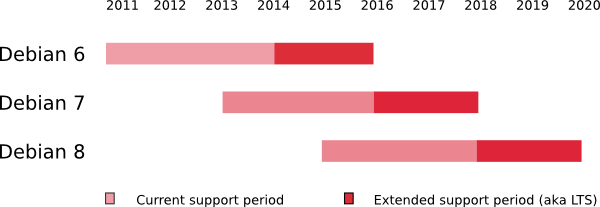
\includegraphics[width=0.7\hsize]{image201506/debian-lts-periods.png}
\end{center}
\caption{LTSのサポート期間}
\end{figure}

\end{frame}

\begin{frame}{LTS(Long Time Support)つづき}

 LTSは無料で利用できる一方、有償サポート契約も用意されている。有償サポート契約をFreexian社と行うと、払った値段に応じて、サポートしてくれるパッケージの選択に関して、要望が通りやすくなるという特典がある。日本の会社様にての契約締結実績はGREE社のみ。
\ \\ 
詳しくは:\\
「Debian Long Term Support」\\
\url{https://www.freexian.com/en/services/debian-lts.html}

\end{frame}

\begin{frame}{debian-security-supportパッケージ}

 debian-security-supportパッケージを導入し、check-support-statusコマンドを実行すると、
現在お使いのDebian機に導入されいているパッケージの脆弱性のサポートについて、サポート切れ、もしくは、何らかの理由により脆弱性対策にあたり制限を加えざるを得なかったもののリストが取れるようになった。

\end{frame}

\begin{frame}{debian-security-supportパッケージ(つづき)}

   動作としては、
\begin{itemize}
\item  /usr/share/debian-security-support/security-support-ended
\item /usr/share/debian-security-support/security-support-limited
\end{itemize}
に記載された、各パッケージのサポート状況に関する制限の情報と、実際に導入されていてるパッケージ名を照合し、制限があるパッケージが見つかった場合は警告を出すという動作。LTSの元では、どこまでパッケージについて、脆弱性対応のサポートがなされているかの確認に便利。

\end{frame}

\begin{frame}{おわりに}

  Debianのコミュニティは、Linux、OSSにまつわる様々な問題点や課題を、コミュニティの力を結集して日夜解決していくのがミッションであり、参加の醍醐味です。日夜、技術的課題、セキュリティ問題も含め、解決・考察し甲斐のある課題が、次から次へと生まれています。

\begin{center}
是非、Debianへのご参加お待ちしております!!
\end{center}

\end{frame}

\section{今後のイベント}
\emtext{今後のイベント}
\begin{frame}{今後のイベント}
\begin{itemize}
 \item 関西エリアDebian勉強会
 \item 東京エリアDebian勉強会(7/某日)
\end{itemize}
\end{frame}

\section{今日の宴会場所}
\emtext{今日の宴会場所}
\begin{frame}{今日の宴会場所}
未定
\end{frame}

\end{document}

;;; Local Variables: ***
;;; outline-regexp: "\\([ 	]*\\\\\\(documentstyle\\|documentclass\\|emtext\\|section\\|begin{frame}\\)\\*?[ 	]*[[{]\\|[]+\\)" ***
;;; End: ***
